%! AP Statistics — Unit 2, Lesson 2.2 — Student Guided Notes
\documentclass[10pt]{article}
\usepackage{apstats-article}
\usepackage{apstats-boxes}

%=============================================================================
\begin{document}

\pageheader{Unit 2, Lesson 2.2}{Guided Notes}
\namedateperiod

\vspace{0.12in}

% ── OBJECTIVE ────────────────────────────────────────────────────────────────
\begin{objectivebox}
\small By the end of this lesson, I will be able to\dots\\[4pt]
\writeline\\[1pt]
\writeline\\[1pt]
\writeline
\end{objectivebox}

\vspace{0.1in}

% ── VOCABULARY ───────────────────────────────────────────────────────────────
\begin{vocabbox}
\termblanklong{Two-way table (contingency table)}
\termblanklong{Joint frequency}
\termblanklong{Marginal frequency}
\termblanklong{Joint relative frequency}
\termblanklong{Conditional relative frequency}
\termblanklong{Association (two categorical variables)}
\end{vocabbox}

\vspace{0.1in}

% ── HOOK ─────────────────────────────────────────────────────────────────────
\begin{hookbox}
\small\textbf{Scenario:} A researcher surveys 240 high school students and records
two variables for each student: (1) grade level --- \textit{Underclassman} (9th/10th) or
\textit{Upperclassman} (11th/12th), and (2) preferred lunch location ---
\textit{Cafeteria}, \textit{Off-campus}, or \textit{Home}.

\vspace{6pt}
\textbf{Statistical question:} \textit{Is there an association between grade level and
lunch preference?}

\vspace{6pt}
\textbf{Discussion:}
\begin{enumerate}[leftmargin=1.5em, itemsep=2pt]
  \item Why can't a single bar chart (one variable) answer this question?\\
        \writeline

  \item What kind of display would let you compare lunch preferences across grade levels?\\
        \writeline
\end{enumerate}
\end{hookbox}

\vspace{0.1in}

% ── BUILDING A TWO-WAY TABLE ─────────────────────────────────────────────────
\begin{notesbox}{Step 1 --- Build the Two-Way Table (UNC-1.P.3)}
\small

\noindent Here are the 240 survey results organized into a two-way table.
Label each part as directed below.

\vspace{8pt}
\renewcommand{\arraystretch}{2.0}
\begin{tabularx}{\linewidth}{@{} l C{2.4cm} C{2.4cm} C{2.2cm} C{2.2cm} @{}}
\rowcolor{sky}
\textbf{Grade Level}
  & \textbf{Cafeteria} & \textbf{Off-campus} & \textbf{Home}
  & \textbf{\color{navy}Row Total} \\
\hline
Underclassman & 54 & 18 & 48 & \blank{1.8cm} \\
Upperclassman & 36 & 42 & 42 & \blank{1.8cm} \\
\hline
\textbf{Column Total} & \blank{1.8cm} & \blank{1.8cm} & \blank{1.8cm} & \blank{1.8cm} \\
\end{tabularx}

\vspace{10pt}

\begin{enumerate}[leftmargin=1.4em, itemsep=4pt]
  \item Fill in the \textbf{row totals} and \textbf{column totals}.
        These are called \textbf{\blank{3cm} frequencies}.

  \item Circle any one interior cell. The count in that cell is called a
        \textbf{\blank{3cm} frequency} because it describes \blank{4cm}.

  \item The grand total is \blank{1.5cm}. This should equal both the sum of row totals
        \emph{and} the sum of column totals --- verify:
        $\blank{1.2cm} + \blank{1.2cm} = \blank{1.2cm}$
\end{enumerate}

\end{notesbox}

\vspace{0.1in}

% ── RELATIVE FREQUENCIES ─────────────────────────────────────────────────────
\begin{notesbox}{Step 2 --- Relative Frequencies (UNC-1.P.4)}
\small
\begin{multicols}{2}

\textbf{Joint relative frequency}\\[3pt]
Formula: $\dfrac{\text{cell count}}{\text{\blank{2cm}}}$

\vspace{6pt}
Example: What fraction of all 240 students are
underclassmen who eat at the cafeteria?
\[
  \frac{\blank{1cm}}{\blank{1cm}} = \blank{2cm}
\]

\columnbreak

\textbf{Conditional relative frequency}\\[3pt]
Formula: $\dfrac{\text{cell count}}{\text{\blank{3cm}}}$

\vspace{6pt}
Example: Among \emph{underclassmen}, what fraction
prefer the cafeteria?
\[
  \frac{\blank{1cm}}{\blank{1cm}} = \blank{2cm}
\]

\end{multicols}

\vspace{6pt}
\textbf{Key distinction:} Joint relative frequency uses the \blank{3cm} total;
conditional relative frequency uses a \blank{3cm} or \blank{3cm} total.
\end{notesbox}

\vspace{0.1in}

% ── CONDITIONAL DISTRIBUTIONS ────────────────────────────────────────────────
\begin{notesbox}{Step 3 --- Conditional Distribution Table}
\small

\noindent Complete the conditional relative frequency table by dividing each cell
by its \textbf{row total}. Round to the nearest percent.

\vspace{8pt}
\renewcommand{\arraystretch}{2.0}
\begin{tabularx}{\linewidth}{@{} l C{2.8cm} C{2.8cm} C{2.8cm} C{1.6cm} @{}}
\rowcolor{sky}
\textbf{Grade Level}
  & \textbf{Cafeteria} & \textbf{Off-campus} & \textbf{Home}
  & \textbf{Total} \\
\hline
Underclassman & \blank{2.2cm} & \blank{2.2cm} & \blank{2.2cm} & 100\% \\
Upperclassman & \blank{2.2cm} & \blank{2.2cm} & \blank{2.2cm} & 100\% \\
\end{tabularx}

\vspace{10pt}
\textbf{Interpretation:} Compare the two rows. Do the conditional distributions look similar
or different? What does that tell you about association?\\[6pt]
\writeline\\[1pt]\writeline
\end{notesbox}

\vspace{0.1in}

% ── SEGMENTED BAR CHART ──────────────────────────────────────────────────────
\begin{notesbox}{Step 4 --- Segmented Bar Chart (UNC-1.P.1, UNC-1.P.2)}
\small
\begin{multicols}{2}

\textbf{Construction steps:}
\begin{enumerate}[leftmargin=1.4em, itemsep=3pt]
  \item Draw two bars (one per grade level) on the
        same scale, each reaching \blank{1cm}\%.
  \item Divide each bar into segments proportional
        to the \blank{3cm} relative frequencies.
  \item Label each segment with the lunch category
        and use a consistent color/pattern key.
\end{enumerate}

\vspace{6pt}
\textbf{Reading the chart:}\\
If the two bars look \textbf{the same} $\to$ \blank{3cm}\\
If the two bars look \textbf{different} $\to$ \blank{3cm}

\columnbreak

\vspace{4pt}
\textbf{Sketch your segmented bar chart here:}

\vspace{0.8in}

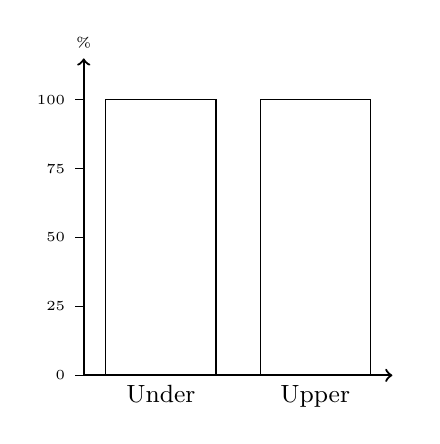
\begin{tikzpicture}[x=1.4cm, y=0.035cm]
  % axes
  \draw[thick,->] (0,0) -- (2.8,0) node[right,font=\small] {};
  \draw[thick,->] (0,0) -- (0,115) node[above,font=\tiny] {\%};
  % y-axis ticks
  \foreach \y in {0,25,50,75,100}{
    \draw (0,\y) -- (-0.08,\y) node[left,font=\tiny] {\y};
  }
  % x-axis labels
  \node[below,font=\small] at (0.7,0) {Under};
  \node[below,font=\small] at (2.1,0) {Upper};
  % empty bar outlines
  \draw (0.2,0) rectangle (1.2,100);
  \draw (1.6,0) rectangle (2.6,100);
\end{tikzpicture}

\end{multicols}

\end{notesbox}

\vspace{0.1in}

% ── ASSOCIATION CONCLUSION ────────────────────────────────────────────────────
\begin{notesbox}{Step 5 --- State the Association Conclusion}
\small

\textbf{Template for an association statement:}\\[4pt]
\textit{``There \blank{1.5cm} [is / is not] evidence of an association between
\blank{3cm} and \blank{3cm}. Among underclassmen, \blank{2cm}\% prefer the cafeteria,
compared to \blank{2cm}\% among upperclassmen. The conditional distributions
\blank{3cm} [are similar / differ], suggesting \blank{3cm}.''}

\vspace{8pt}
\textbf{Write your own conclusion using the data from Step 3:}\\[4pt]
\writeline\\[1pt]\writeline\\[1pt]\writeline

\end{notesbox}

\vspace{0.1in}

% ── CONNECTIONS ───────────────────────────────────────────────────────────────
\begin{spiralbox}
\small
\begin{multicols}{2}

\textbf{How this connects:}
\begin{itemize}[itemsep=3pt]
  \item Lesson 2.1: we asked whether an association exists
        $\to$ today: we build the displays to answer that question
  \item Lesson 2.3: we \emph{quantify} the association with
        statistics (difference in proportions, relative risk)
  \item Unit 8: chi-square test --- is the association statistically significant?
\end{itemize}

\columnbreak

\textbf{Big Idea --- write in your own words:}\\
\textit{Why do we use conditional (not joint) relative
frequencies to check for association?}\\[2pt]
\writeline\\[1pt]\writeline\\[1pt]\writeline

\end{multicols}
\end{spiralbox}

\vspace{0.1in}

\begin{notesbox}{Additional Notes}
\vspace{0pt}
\writeline\\\writeline\\\writeline\\\writeline\\\writeline\\\writeline
\end{notesbox}

\end{document}
